\documentclass[a4paper]{article}
\usepackage{graphicx}
\usepackage{float}
\author{Hein van Beers, Jeroen van Hoof}
\title{Automated Reasoning\\
	 \large Practical assignment, Part I}
\begin{document}
	\maketitle
	
	\section*{Problem 1: Delivery for magic factory}
	Satisfying all constraints, find the maximum number of pallets of prittles that can be delivered, and show how for that number all pallets may be divided over the six trucks.

	
	\section*{Solution:}
	We generalize this problem to $n$ trucks. For each pallet place in a truck we introduce five variables, one for each type of building block. We have eight pallet places per truck, so we introduce $8*5*n = 40*n$ variables $p_{ijk}$ for $i = 1,\ldots,n$, $j = 1,\ldots,8$ and $k = 1,\ldots,5$ where for every $i,j,k$ the value of $p_{ijk}$ will be true if and only if a pallet of building block type $k$ will be put on pallet position $j$ in truck $i$.
	
	As the weight of each of the $n$ trucks may not exceed the capacity of 7800 kg, we express this by the formula
\[ \bigwedge_{i=1}^n (\sum_{k=1}^5 (\sum_{j=1}^8 (f(p_{ijk})*w_k)) \leq 7800).\]
Where $f(p_{ijk}) = 1$ if $p_{ijk}$ is equal to true and 0 otherwise. Also $w_k$ is the weight of a pallet of type $k$. In the table below you can see the weights of the different types of pallets.

\begin{table}[H]
\centering
\caption{Weights of the different types of pallets}
\label{my-label}
\begin{tabular}{c|c|c}
\textbf{Pallet type} & \textbf{Corresponding k} & \textbf{Weight (kg)} \\ \hline
Nuzzles              & 1                        & 700                  \\ \hline
Prittles             & 2                        & 800                  \\ \hline
Skipples             & 3                        & 1000                 \\ \hline
Crottles             & 4                        & 1500                 \\ \hline
Dupples              & 5                        & 100                 
\end{tabular}
\end{table}

	As prittles and crottles are not allowed to be put in the same truck, that is, for every two distinct positions $j,m$ in truck $i$ it is not allowed that both $p_{ij2}$ and $p_{im4}$ are true. This is expressed by the formula
\[ \bigwedge_{i=1}^n (\neg (\bigvee_{j=1}^8 p_{ij2}) \vee \neg (\bigvee_{m=1}^8 p_{im4})).\]

Next we assume that the first two trucks are cooled, so pallets of skipples cannot be placed in trucks 3 upto and including $n$. We express this by the formula
\[ \bigwedge_{i=3}^n \bigwedge_{j=1}^8 \neg p_{ij3}.\]

No two pallets of the type dupples may be placed in the same truck, that is, for every two distinct positions $j,m$ in truck $i$ it is not allowed that both $p_{ij5}$ and $p_{im5}$ are true. This is expressed by the formula
\[ \bigwedge_{i=1}^n \bigwedge_{j,m:1 \leq j < m \leq 8} \neg p_{ij5} \vee \neg p_{im5}.\]

Similarly, we also need the requirement that at most one variable is set to true per pallet position in a truck. So for every two distinct pallet types $k,m$ on position $j$ in truck $i$ it is not allowed that both $p_{ijk}$ and $p_{ijm}$ are true. This is expressed by the formula
\[ \bigwedge_{i=1}^n \bigwedge_{j=1}^8 \bigwedge_{k,m:1 \leq k < m \leq 5} \neg p_{ijk} \vee \neg p_{ijm}.\]

Finally, we consider the requirements of the demands. As the amount of pallets that need to be delivered for each pallet type is given, except for the prittles, we can express this by the formula
\[ \bigwedge_{k=1}^5 ( \sum_{i=1}^n ( \sum_{j=1}^8 f(p_{ijk}) ) = a_k).\]
Where $f(p_{ijk}) = 1$ if $p_{ijk}$ is equal to true and 0 otherwise. And $a_k$ is the amount of a pallets of type $k$ that need to be delivered. In the table below you can see the amount for each type of pallet.

\begin{table}[H]
\centering
\caption{Demand of each type of pallets}
\label{my-label}
\begin{tabular}{c|c|c}
\textbf{Pallet type} & \textbf{Corresponding k} & \textbf{Demand (pallets)} \\ \hline
Nuzzles              & 1                        & 4                  		\\ \hline
Prittles             & 2                        & ?                  		\\ \hline
Skipples             & 3                        & 8                 		\\ \hline
Crottles             & 4                        & 10                 		\\ \hline
Dupples              & 5                        & 5                 
\end{tabular}
\end{table}

For getting the answer to the maximization problem, we just try different values for the amount of pallets of prittles that need to be delivered and see if we get a solution. When we find a solution for a value $x$ for the amount of prittles that we deliver and we cannot find a solution for value $x+1$, we know that $x$ is the maximum number of pallets of prittles that can be delivered.

After trying several values, we found that 18 pallets of prittles is the maximum amount we can deliver, since the program does not yield a solution for 19 pallets of prittles.

The total formula now consists of the conjunction of all these ingredients, that is,
\[ \bigwedge_{i=1}^n (\sum_{k=1}^5 (\sum_{j=1}^8 (p_{ijk}*w_k)) \leq 7800) \;\; \wedge \]
\[ \bigwedge_{i=1}^n (\neg (\bigvee_{j=1}^8 p_{ij2}) \vee \neg (\bigvee_{m=1}^8 p_{im4})) \;\; \wedge \]
\[ \bigwedge_{i=3}^n \bigwedge_{j=1}^8 (\neg p_{ij3}) \;\; \wedge \]
\[ \bigwedge_{i=1}^n \bigwedge_{j,m:1 \leq j < m \leq 8} (\neg p_{ij5} \vee \neg p_{im5}) \;\; \wedge \]
\[ \bigwedge_{i=1}^n \bigwedge_{j=1}^8 \bigwedge_{k,m:1 \leq k < m \leq 5} (\neg p_{ijk} \vee \neg p_{ijm}) \;\; \wedge \]
\[ \bigwedge_{k=1}^5 ( \sum_{i=1}^n ( \sum_{j=1}^8 p_{ijk} ) = a_k) \]


This formula is easily expressed in SMT syntax, for instance, for
$n=6$ one can generate

{\footnotesize

{\tt (benchmark Assignment1.smt}

{\tt :logic QF\_LIA}

{\tt :extrapreds (}

{\tt ;Truck 1 }

{\tt (p111) (p112) (p113) (p114) (p115) }

{\tt (p121) (p122) (p123) (p124) (p125) }

{\tt (p131) (p132) (p133) (p134) (p135) }

{\tt (p141) (p142) (p143) (p144) (p145) }

{\tt (p151) (p152) (p153) (p154) (p155) }

{\tt (p161) (p162) (p163) (p164) (p165) }

{\tt (p171) (p172) (p173) (p174) (p175) }

{\tt (p181) (p182) (p183) (p184) (p185) }

{\tt ;Truck 2 }

{\tt (p211) (p212) (p213) (p214) (p215) }

{\tt (p221) (p222) (p223) (p224) (p225) }

$\cdots \cdots$

{\tt )}

{\tt :formula}

{\tt   (and}

{\tt (<= (+ }

{\tt (* (ite p111 1 0) 700) $\cdots$ (* (ite p181 1 0) 700)}

{\tt (* (ite p112 1 0) 800) $\cdots$ (* (ite p182 1 0) 800)}

$\cdots \cdots$

{\tt (* (ite p115 1 0) 100) $\cdots$ (* (ite p185 1 0) 100)}

{\tt ) 7800)}

$\cdots \cdots$

{\tt (or }

{\tt (not (or p112 p122 p132 p142 p152 p162 p172 p182)) }

{\tt (not (or p114 p124 p134 p144 p154 p164 p174 p184)) }

{\tt ) }

$\cdots \cdots$

{\tt )) }
}

Applying {\tt yices -m -smt Assignment1.smt} yields the following result
within a fraction of a second:

{\footnotesize

{\tt sat }

{\tt (= p185 false)}

{\tt (= p445 false)}

{\tt (= p213 true)}

{\tt (= p214 false)}

{\tt (= p452 false)}

{\tt (= p233 true)}

{\tt (= p435 false)}

{\tt (= p474 true)}

{\tt (= p623 false)}

{\tt (= p531 true)}

{\tt (= p662 false)}

$\cdots \cdots$ }

The values that are are true for each truck are 
\[p113, p123, p133, p141, p155, p163, p174, p184 \]
\[p212, p223, p232, p243, p252, p262, p273, p283 \]
\[p312, p322, p332, p342, p352, p362, p375, p382 \]
\[p412, p422, p432, p442, p452, p465, p472, p482 \]
\[p514, p521, p534, p544, p554, p565, p571 \]
\[p615, p621, p634, p644, p674, p684 \]
Expressed in a picture this yields

\begin{figure}[H]
			\centering
				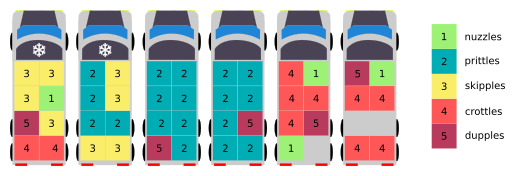
\includegraphics[scale=1]{trucks.png}
			\caption{Placement of pallets on truck. The first two trucks have facility for cooling skipples.}
		\end{figure}

We check that indeed all requirements are satisfied and we also see that the amount of pallets of prittles we can deliver is 18, since the program does not yield a solution for 19 pallets of prittles.

{\bf Remark:} 

Our formula contains some redundancy: the requirement that every
row contains exactly one queen implies that there are exactly $n$
queens in total. By expressing that every column contains at least
one queen, from this property one concludes that also every column
contains at most one queen. We chose for this redundancy for
keeping the symmetry in the solution, and also following the
general strategy that introducing redundancy is often good for
efficiency.

\vspace{3mm}

{\bf Generalization:} 

As we generalized our approach for $n$ rather than 8, it is
interesting to see what happens for other values of $n$. For $n
> 10$ we have to take care of the notation: if we keep the
notation then it is not clear whether {\tt p111} represents 
$p_{1,11}$ or $p_{11,1}$. This is solved by putting an extra 
symbol between the two numbers. 

For $n=3$ the resulting formula is unsatisfiable, showing that
there is no solution. For $n = 4,5,6,\ldots$ the formula is
satisfiable, by which is a solution of the problem is found.
Efficiency is not a problem: for $n = 60$ there are 3600
variables and the formula consists of over 350,000 clauses, but 
still {\tt yices} succeeds in finding a solution within a few
seconds.
	\section*{Problem 2: Placing components on a power grid}
	To identify each component, we have named them $a, b, ... h$, with sizes $9 \times 7$, $12 \times 6$, $10 \times 7$, $18 \times 5$, $20 \times 4$, $10 \times 6$, $8 \times 6$ and $10 \times 8$. Furthermore, we named the power components $i, j, k$. 
	The specification that each component can be turned to $90^{\circ}$, can be simplified to swapping the x and y dimensions of a component with each other. For each component, we introduce predicates $a\_turned, b\_turned, ..., k\_turned$ to indicate rotation, and $a\_lx, a\_ly, b\_lx, b\_ly, ..., k\_lx, k\_ly,$ for the lengths and widths of $a, b, ..., k$. So the dimensions of each component are determined as follows:

	{\tt (= a\_lx (ite a\_turned 7 9))}
	
	{\tt (= a\_ly (ite a\_turned 9 7))}
	
	{\tt ...}
	
	\noindent We identify the origin of each component, with predicates $a\_ox, a\_oy, b\_ox, b\_oy, ..., k\_ox, k\_oy$ to denote x-origins and y-origins. To specify the size of the chip, we have to make sure that all components are within the limits of the length and width:
	
	{\tt (<= (+ a\_lx a\_ox) 29)}
	
	{\tt (>= a\_ox 0)}
	
	{\tt (<= (+ a\_ly a\_oy) 22)}
	
	{\tt (>= a\_oy 0)}
	
	{\tt ...}
	
	\noindent We must also make sure that none of the components overlap. To make sure that two components, a and b, do not overlap, one of four statements must hold:
	\begin{itemize}
		\item \textbf{b} is right of \textbf{a} $\Leftrightarrow a\_ox >= b\_x + b\_lx$
		\item \textbf{b} is left of \textbf{a} $\Leftrightarrow b\_ox >= a\_ox + a_lx$
		\item \textbf{b} is below \textbf{a} $\Leftrightarrow a\_oy >= b\_oy + b\_ly$
		\item \textbf{b} is above \textbf{a} $\Leftrightarrow b\_oy >= a\_oy + a\_ly$
	\end{itemize}
	In SMT:
	
	{\tt (or (>= a\_ox (+ b\_ox b\_lx)) (>= b\_ox (+ a\_ox a\_lx)) (>= a\_oy (+ b\_oy b\_ly)) (>= b\_oy (+ a\_oy a\_ly)) )}\\
	\noindent We need to repeat this statement for every pair, in order to make sure no two components overlap each other.\\
	
	\noindent The next requirement is that every component needs to be adjacent to a power component. More formally, when we have $n$ regular components and $m$ power components, we have for each regular component $c$ and power component $p$:
	
	$$\bigwedge_{c=1}^n \bigvee_{p=1}^m c\ adjacent\ to\ p $$
	
	\noindent where $c\ adjacent\ to\ p $ is defined as:
	\begin{itemize}
	\item If side $p$ is left or right of $c$, then $p\_oy + p\_ly <= c\_oy >= p\_oy - c\_ly$
	\item If side $p$ is above or below $c$, then $p\_ox + p\_lx <= c\_ox >= p\_ox - c\_lx$
	\end{itemize}
	
	\noindent In SMT:
	
	{\tt ; B is adjacent to a Powerchip}
	
	{\tt (or}
	
	{\tt ; A adjacent to I}
	
	{\tt (and}
	
	{\tt (= a\_ox (+ i\_ox i\_lx)) (>= a\_oy (- i\_oy a\_ly)) (<= a\_oy (+ i\_oy i\_ly)))}
	
	{\tt (and}
	
	{\tt (= i\_ox (+ a\_ox a\_lx)) (>= i\_oy (- a\_oy i\_ly)) (<= i\_oy (+ a\_oy a\_ly)))}
	
	{\tt (and }
	
	{\tt (= a\_oy (+ i\_oy i\_ly)) (>= a\_ox (- i\_ox a\_lx)) (<= a\_ox (+ i\_ox i\_lx)))}
	
	{\tt (and}
	
	{\tt (= i\_oy (+ a\_oy a\_ly)) (>= i\_ox (- a\_ox i\_lx)) (<= i\_ox (+ a\_ox a\_lx)))}
	
	{\tt ; A next to J}
	
	{\tt ...}
	
	{\tt )}

	{\tt ; B is adjacent to a Powerchip}

	{\tt ...}\\
	
	\noindent The last requirement was that the centers of any two power components should differ at least 17 in either the x direction or the y direction (or both).\\
	Take arbitrary power components $i$ and $j$, then we have:
	
	$$\mid(i\_ox + 0.5 * i\_lx) - (j\_ox + 0.5 * j\_lx)\mid\ >= 17\ \vee$$
	$$\mid(i\_oy + 0.5 * i\_ly) - (j\_oy + 0.5 * j\_ly)\mid\ >= 17 $$
	
	\begin{figure}[H]
		\centering
			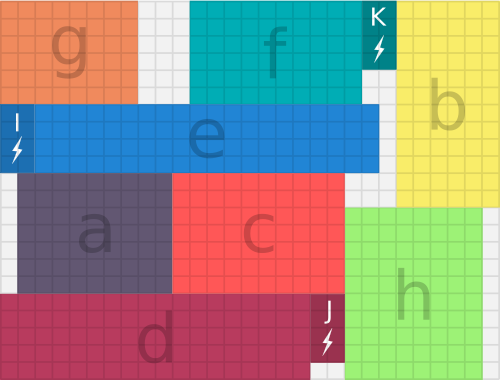
\includegraphics[scale=0.7]{power-grid-3.png}
		\caption{Placement of components on chip.}
	\end{figure}
	\section{Problem 3}
	\begin{figure}[H]
		\centering
			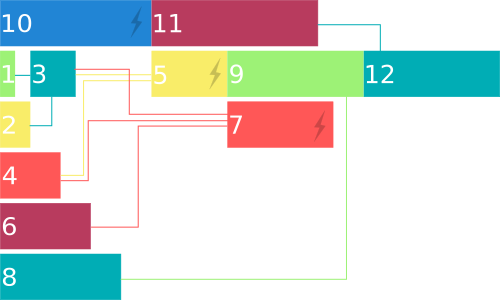
\includegraphics[scale=0.7]{timeline.png}
		\caption{Time-line of process execution. Connected and horizontal adjacent processes depend on each other, special processes are marked with a sign.}
	\end{figure}
	
\end{document}